% small.tex
\documentclass{beamer}
\usetheme{default}
\usepackage{amsmath, amsfonts, amssymb, amsthm}
\usepackage{graphicx}

\newcommand{\afe}{\frac{\alpha}{Fe}}
\newcommand{\feh}{\frac{Fe}{H}}

\newcommand{\eqn}[1]{\begin{align*}
#1
\end{align*}}
\newcommand{\eqnl}[2]{\begin{align} \label{#1}
#2
\end{align}}



\newcommand{\vect}[1]{\boldsymbol{\mathbf{#1}}}
\newcommand{\degree}[1]{${#1}^{\circ}$}
\newcommand{\highlight}{ \rowcolor{lightgrass} }
\newcommand{\script}[1]{\mathcal{#1}}
\newcommand{\bl}{\big\{}
\newcommand{\br}{\big\}}
\newcommand{\Bl}{\Big\{}
\newcommand{\Br}{\Big\}}
\newcommand{\argmax}{\operatornamewithlimits{argmax}}
\newcommand{\eqnset}[4]{
\[ #1 = #2 \left\{ \begin{array}{#3}
        #4
\end{array} \right. \] 
}




\newcommand{\vz}{\vect{z}}
\newcommand{\vx}{\vect{x}}
\newcommand{\vy}{\vect{y}}
\newcommand{\vp}{\vect{\pi}}
\newcommand{\vph}{\hat{\vect{\pi}}}
\newcommand{\vpmle}{\hat{\vect{\pi}}_\text{MLE}}
\newcommand{\sumn}{\sum^n_{i=1}}
\newcommand{\summ}{\sum^m_{j=1}}
\newcommand{\summo}{\sum^{m-1}_{j=1}}
\newcommand{\sumg}{\sum^g_{j=1}}
\newcommand{\sumk}{\sum^m_{k=1}}
\newcommand{\fab}{f_j}
\newcommand{\llp}{L(\vp)}

\newcommand{\vpg}{\vp^{\prime}}
\newcommand{\vpgh}{\hat{\vp}^{\prime}}
\newcommand{\llpp}{L(\vpg)}
\newcommand{\llpph}{L(\vpgh)}

\begin{document}




%%%%%%%%%%%%%%%%%%%%%
\begin{frame}{Link between curves and M theoretical distributions}
	
	(Duane will cover this part I think)
	
	
	Partition the mass and accretion time into $m$ combinations of $\mathcal{M},\mathcal{T}$ where
	
	\eqn{
		\text{Sat. stellar mass:} \hspace{3mm} \bigcup \mathcal{M}_j &= [0, 10^9] M_{\bigodot}  		\\
		\text{Accretion time:} \hspace{3mm} \bigcup \mathcal{T}_j &= [0, 14] \text{Gyr} 
	}
	\eqn{
		f_j(x,y) &= P(x,y|\text{Mass}\in \mathcal{M}_j, \text{Accretion time}\in \mathcal{T}_j)
	}

\end{frame}


%%%%%%%%%%%%%%%%%%%%%
\begin{frame}{A generative finite mixture model}
	
	
		
	\begin{figure}
			\begin{center}
				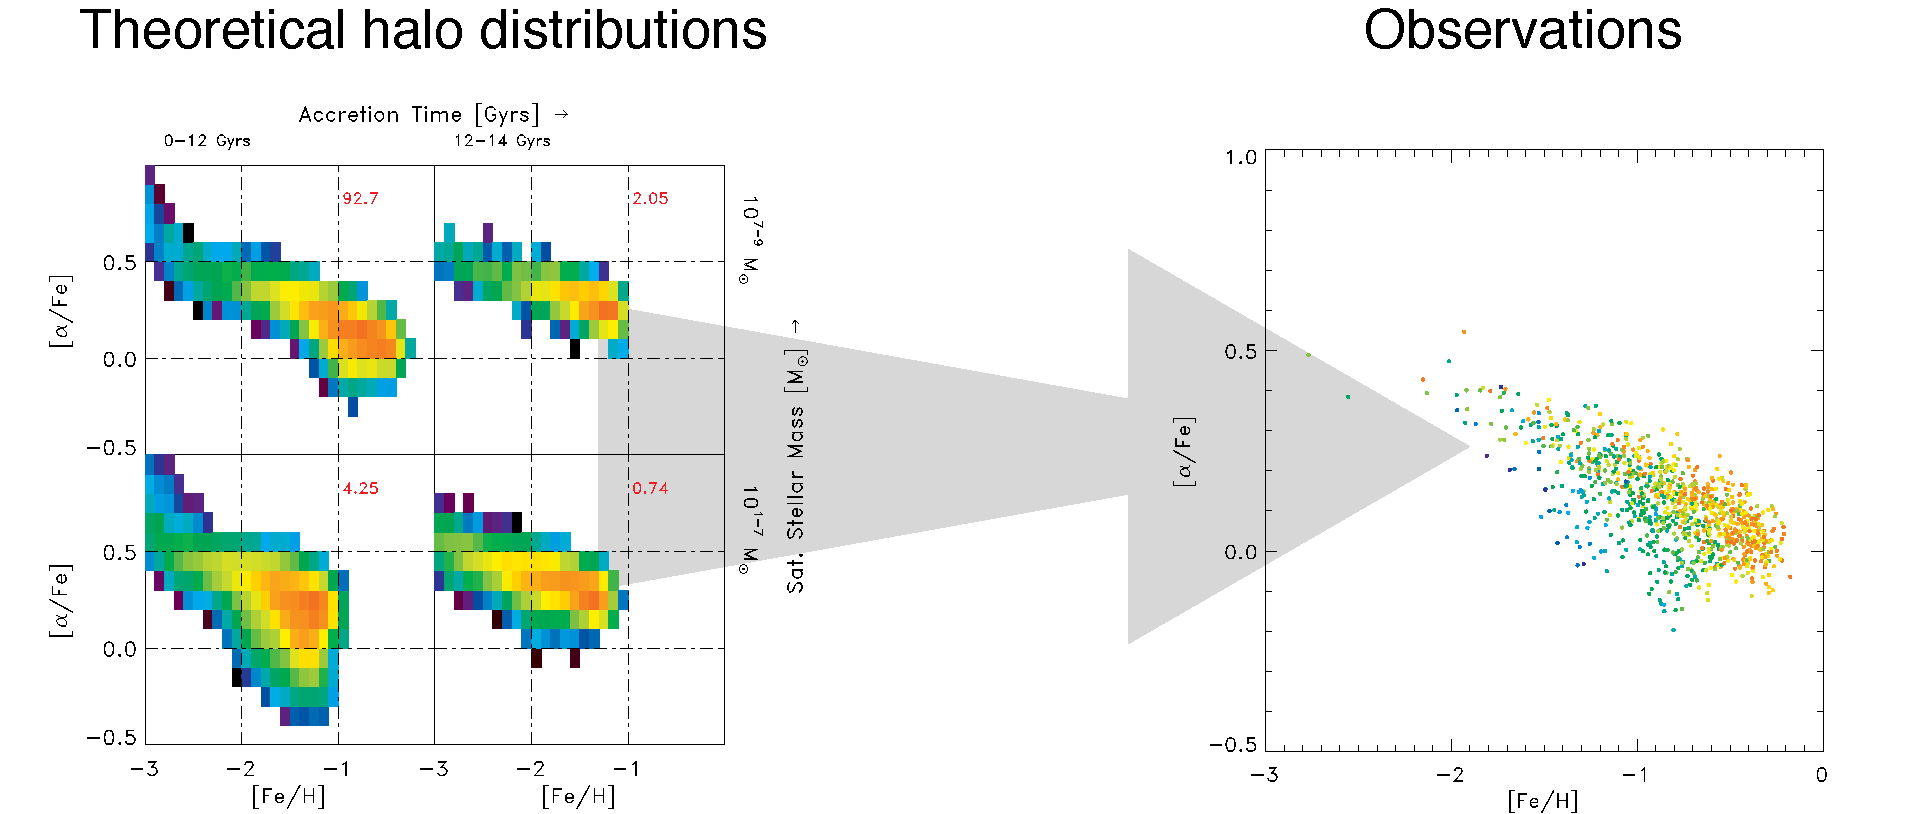
\includegraphics[width=\textwidth]{denstoobs.pdf}
			\end{center}
	\end{figure}
	
	\eqn{
		\Bigg[\feh,\afe\Bigg]_{i=1}^{N} \text{i.i.d} \sim F(x,y) = \sum^m_{j=1} \pi_j f_j(x,y)
	}	
	
\end{frame}







%%%%%%%%%%%%%%%%%%%%%
\begin{frame}{Finding the mixing proportions $\vect{\pi}$}
	
	Unfortunately the maximum likelihood estimate of the mixing proportions,
	\eqn{
		\vph_{\text{MLE}} &= \argmax_{\vp} L(\vect{\pi})
	}
	
	
	is intractable as our model
	
	\eqn{
		F(x,y) &= \sum^m_{j=1} \pi_j f_j(x,y)
	}
	
	has a log likelihood of
	\eqn{
		L(\vect{\pi}) &= \sumn \log \Big( \summ \pi_j \fab(x_i,y_i)  \Big)
	}
	
	
	
	
\end{frame}







%%%%%%%%%%%%%%%%%%%%%
\begin{frame}{Adding the latent variable $\vect{z}$}
	
	Suppose we knew which $f_j$ each observation came from:
	
	\eqn{
		z_{ij} 	= \hspace{1mm} & 1  \hspace{4mm} \text{if} \hspace{1mm} (x_i,y_i) \sim f_j	\\
				& 0 \hspace{4mm} \text{otherwise}
	}
	
	
	The log likelihood can then be expressed as
	
	\eqn{
		L(\vect{\pi}) &= \sumn \summ z_{ij}  \log \bl \pi_j  \fab(x_i,y_i) \br
	}
	
	The addition of the latent variable $\vect{z}$ actually makes things easier by allowing us to use expectation maximization to estimate of $\vp$. 
	
	
\end{frame}










%%%%%%%%%%%%%%%%%%%%%
\begin{frame}{Finding $\vph$ using expectation maximization}
	
	\eqn{
		\vph^{(t)} &= \argmax_{\vp} \mathbb{E}_{\vect{z}| \vx,\vy,\vph^{(t-1)} }\Big[\llp \Big]   
	}
	
	At each time $t$, the estimate for $\vp$ is the argmax of the expected value of the likelihood, given the data and the estimate of $\vp$ from the previous time.
	
	\begin{itemize}
		\item First we find the expected value of $\llp$ using the current estimate of the latent variable
		\item $\vph^{(t)}$ is the $\argmax_{\vp}$ of this expectation
		\item We repeat until $\llp$ stabilizes
	\end{itemize}
	
	
	
	
\end{frame}






%%%%%%%%%%%%%%%%%%%%%
\begin{frame}{Find the expected value of $L(\vect{\pi})$ using the current estimate of the latent variable}
	
	The expected value of $\llp$, with respect to the conditional distribution of $\vect{z}$, given observed data and $\vp^{(t-1)}$ is
	
	\eqn{
		\mathbb{E}_{\vp}\Big[\llp \big| \vx,\vy \Big] &= \sumn \summ \mathbb{E}_{\vp}\big[z_{ij}|x_i,y_i\big] \bl \log \fab(x_i,y_i) + \log \pi_j  \br
	}
	
	Since $z_{ij}$ is an indicator, its expected value is simply the probability that data point $i$ comes from model $j$
	\eqn{
		\mathbb{E}_{\vp}\Big[  z_{ij} | x_i, y_i \Big]	&= \text{Pr}_{\vp}(z_{ij}|x_i,y_i)	\\
										&= \frac{p(x_i,y_i|z_{ij}=1)p(z_{ij}=1)}{p(x_i,y_i)}	\\
										&=  \frac{\pi_j \fab(x_i,y_i)  }{\summ \pi_j \fab(x_i,y_i)}
	}
	
	
		
	
\end{frame}















%%%%%%%%%%%%%%%%%%%%%
\begin{frame}{Find the $\argmax_{\vp}$ of this expectation}
	
		
	Now that we have the expected value of $\llp$ with respect to the conditional distribution of $\vect{z}$, we need only evaluate
	
	
	\eqn{
		\vph^{(t)} &= \argmax_{\vp} \mathbb{E}\Big[\llp \big| \vx,\vy,\vph^{(t-1)} \Big]   
	}
	
	Let
	
	\eqn{
		\hat{\vect{w}}^{(t)} = \mathbb{E}_{\vp}\Big[  z_{ij} | x_i, y_i \Big]
	}
	
	Accounting for the $m-1$ free parameters of $\vp$, differentiation proceeds, for $k=1,\ldots,m-1$, as:
	
	\eqn{
		\frac{\partial}{\partial \pi_k} \mathbb{E}\Big[\llp \big| \vect{x},\vect{y}\Big]   &=      \sumn \Bl  w^{(t-1)}_{ik} \frac{1}{\pi_k} - w^{(t-1)}_{im} \frac{1}{1-\pi_1-\ldots-\pi_{m-1}}   \Br
	}
	\eqn{
		\frac{1}{\pi_k} \sumn w_{ik}^{(t-1)} &= \frac{1}{1-\pi_1-\ldots-\pi_{m-1}} \sumn w_{im}^{(t-1)}
	}
	
	
\end{frame}















%%%%%%%%%%%%%%%%%%%%%
\begin{frame}{Find the $\argmax_{\vp}$ of this expectation}
	
	
	Consequently
	\eqnset{\hat{\pi}^{(t)}_k }{}{ll}{
		\frac{\sumn w^{(t-1)}_{ij}}{n}			& k=1,\ldots,m-1	\\
		\vspace{1mm} & \\
		1-\pi_1-\ldots-\pi_{m-1}		& k=m
	}
	
		Where
	\eqnset{w^{(t+1)}_{ij}}{}{ll}{
		\frac{\displaystyle\pi^{(t)}_{j} \fab(x_i,y_i)}{\displaystyle\sumk \pi^{(t)}_{k}f_k(x_i,y_i)}				& j=1,\ldots,m-1	\\
		\vspace{1mm} & \\
		1 - w_{i1} - \ldots - w_{i,m-1}		& j=m
	}
	
\end{frame}





%%%%%%%%%%%%%%%%%%%%%
\begin{frame}{Simulations}
	
	
	
	
	\begin{itemize}
		\item Generated observations from one halo and multiple halos
		
		\item Used a 5x5 grid ($m=25$), and several 2x2 grids ($m=4$)
		\begin{itemize}
			\item 5x5 grid did not work for some halo realizations
			\item 2x2 grid reliably converged on the correct mixing proportions
		\end{itemize}
	\end{itemize}
	
	
	
	\begin{figure}
			\begin{center}
				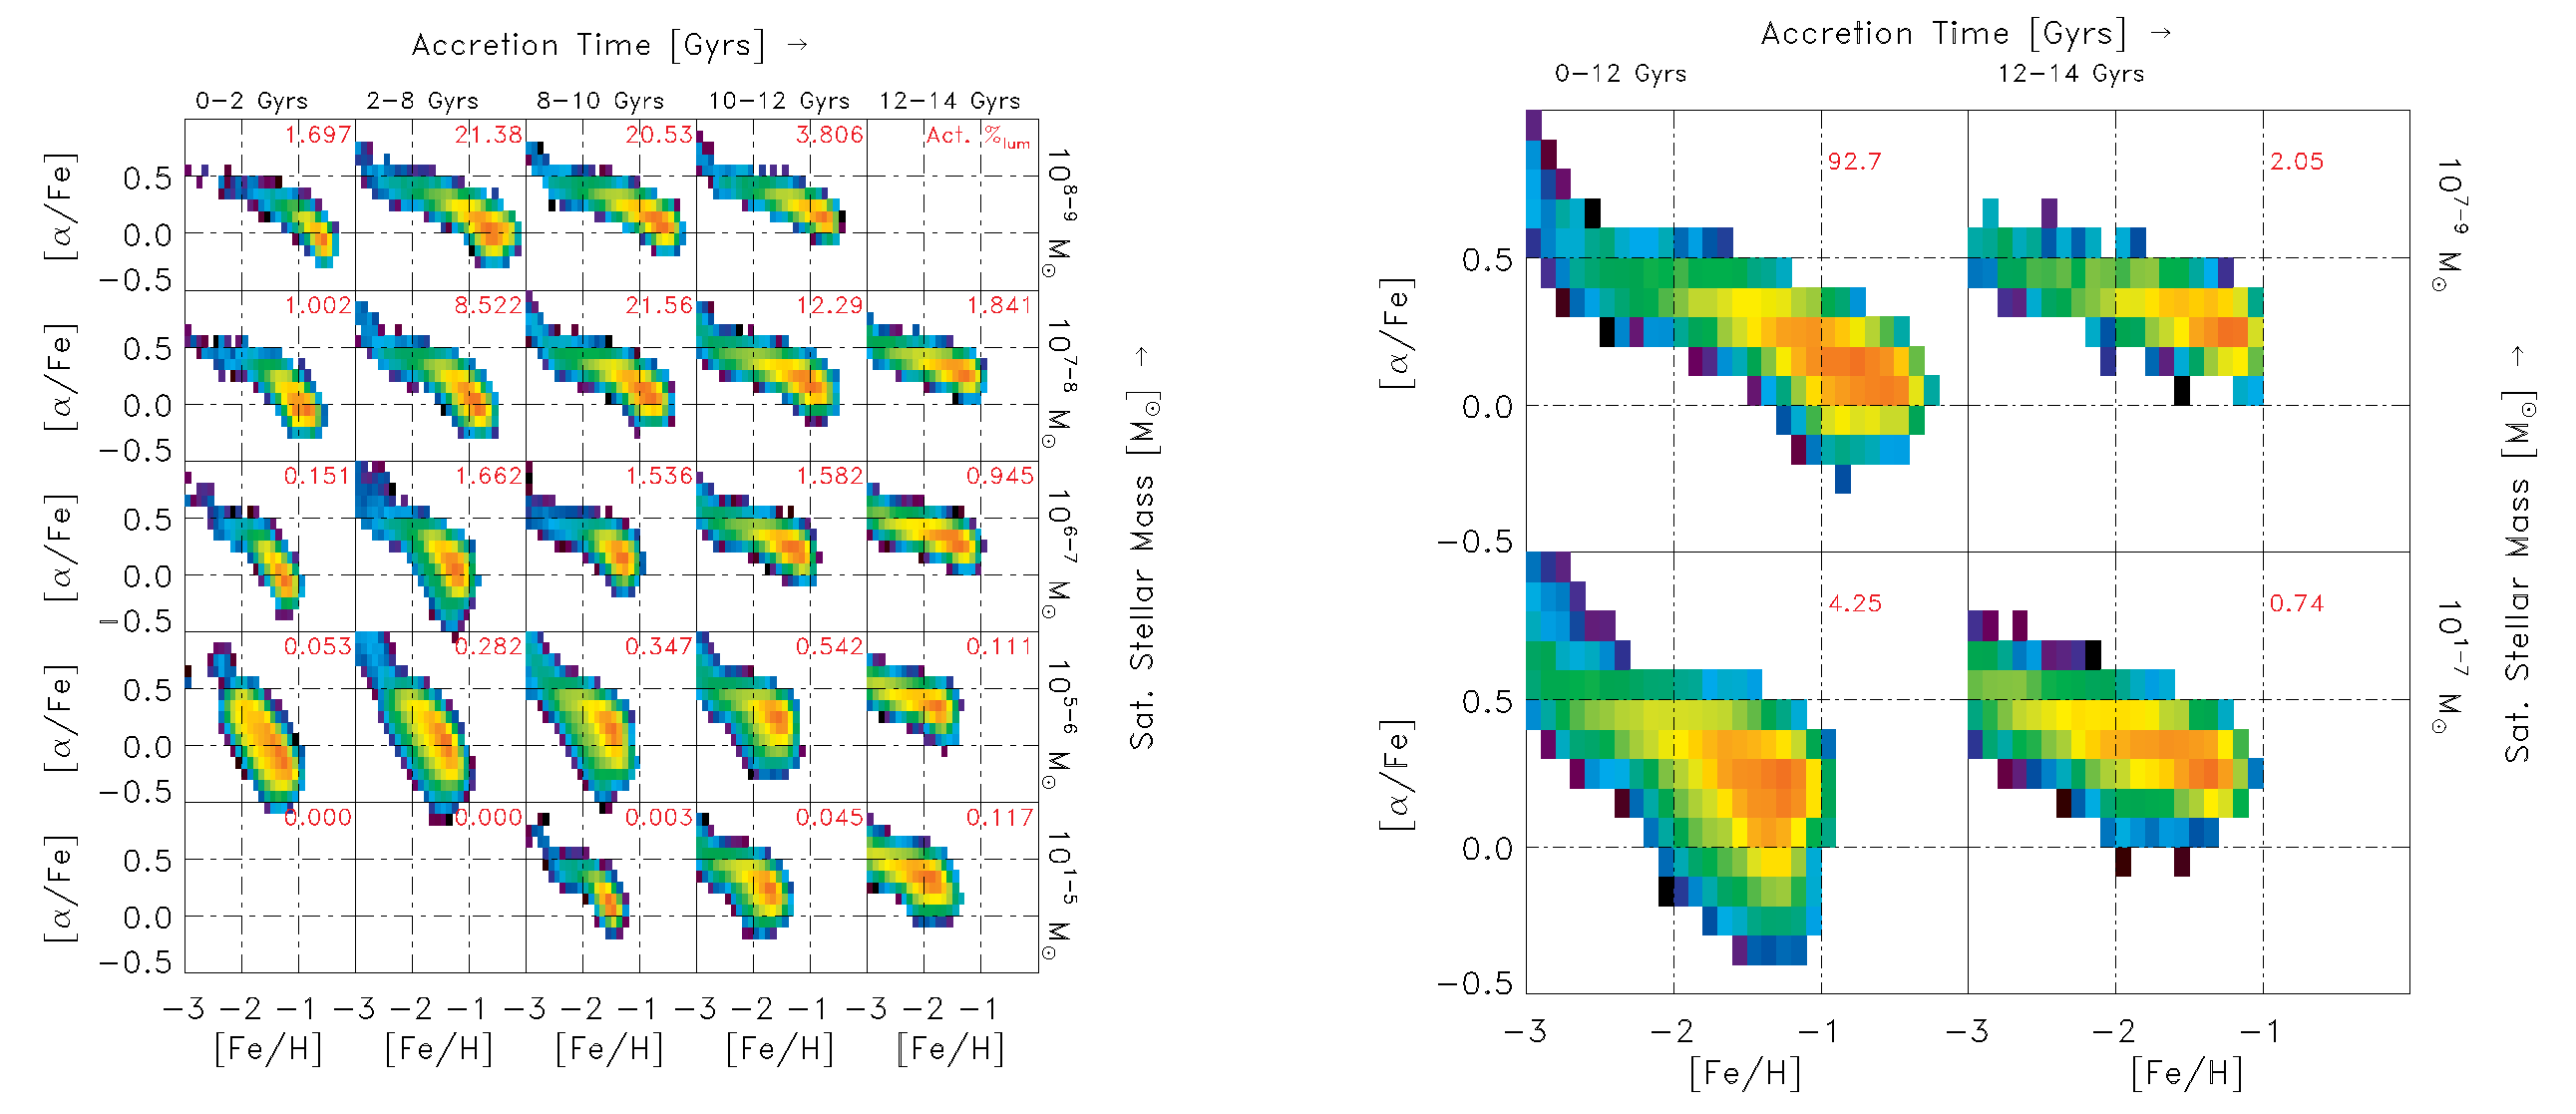
\includegraphics[width=\textwidth]{ourdens.pdf}
			\end{center}
	\end{figure}
	
	
	
	
\end{frame}






%%%%%%%%%%%%%%%%%%%%%
\begin{frame}{EM formation history for $m$=25}
	
	\begin{figure}
			\begin{center}
				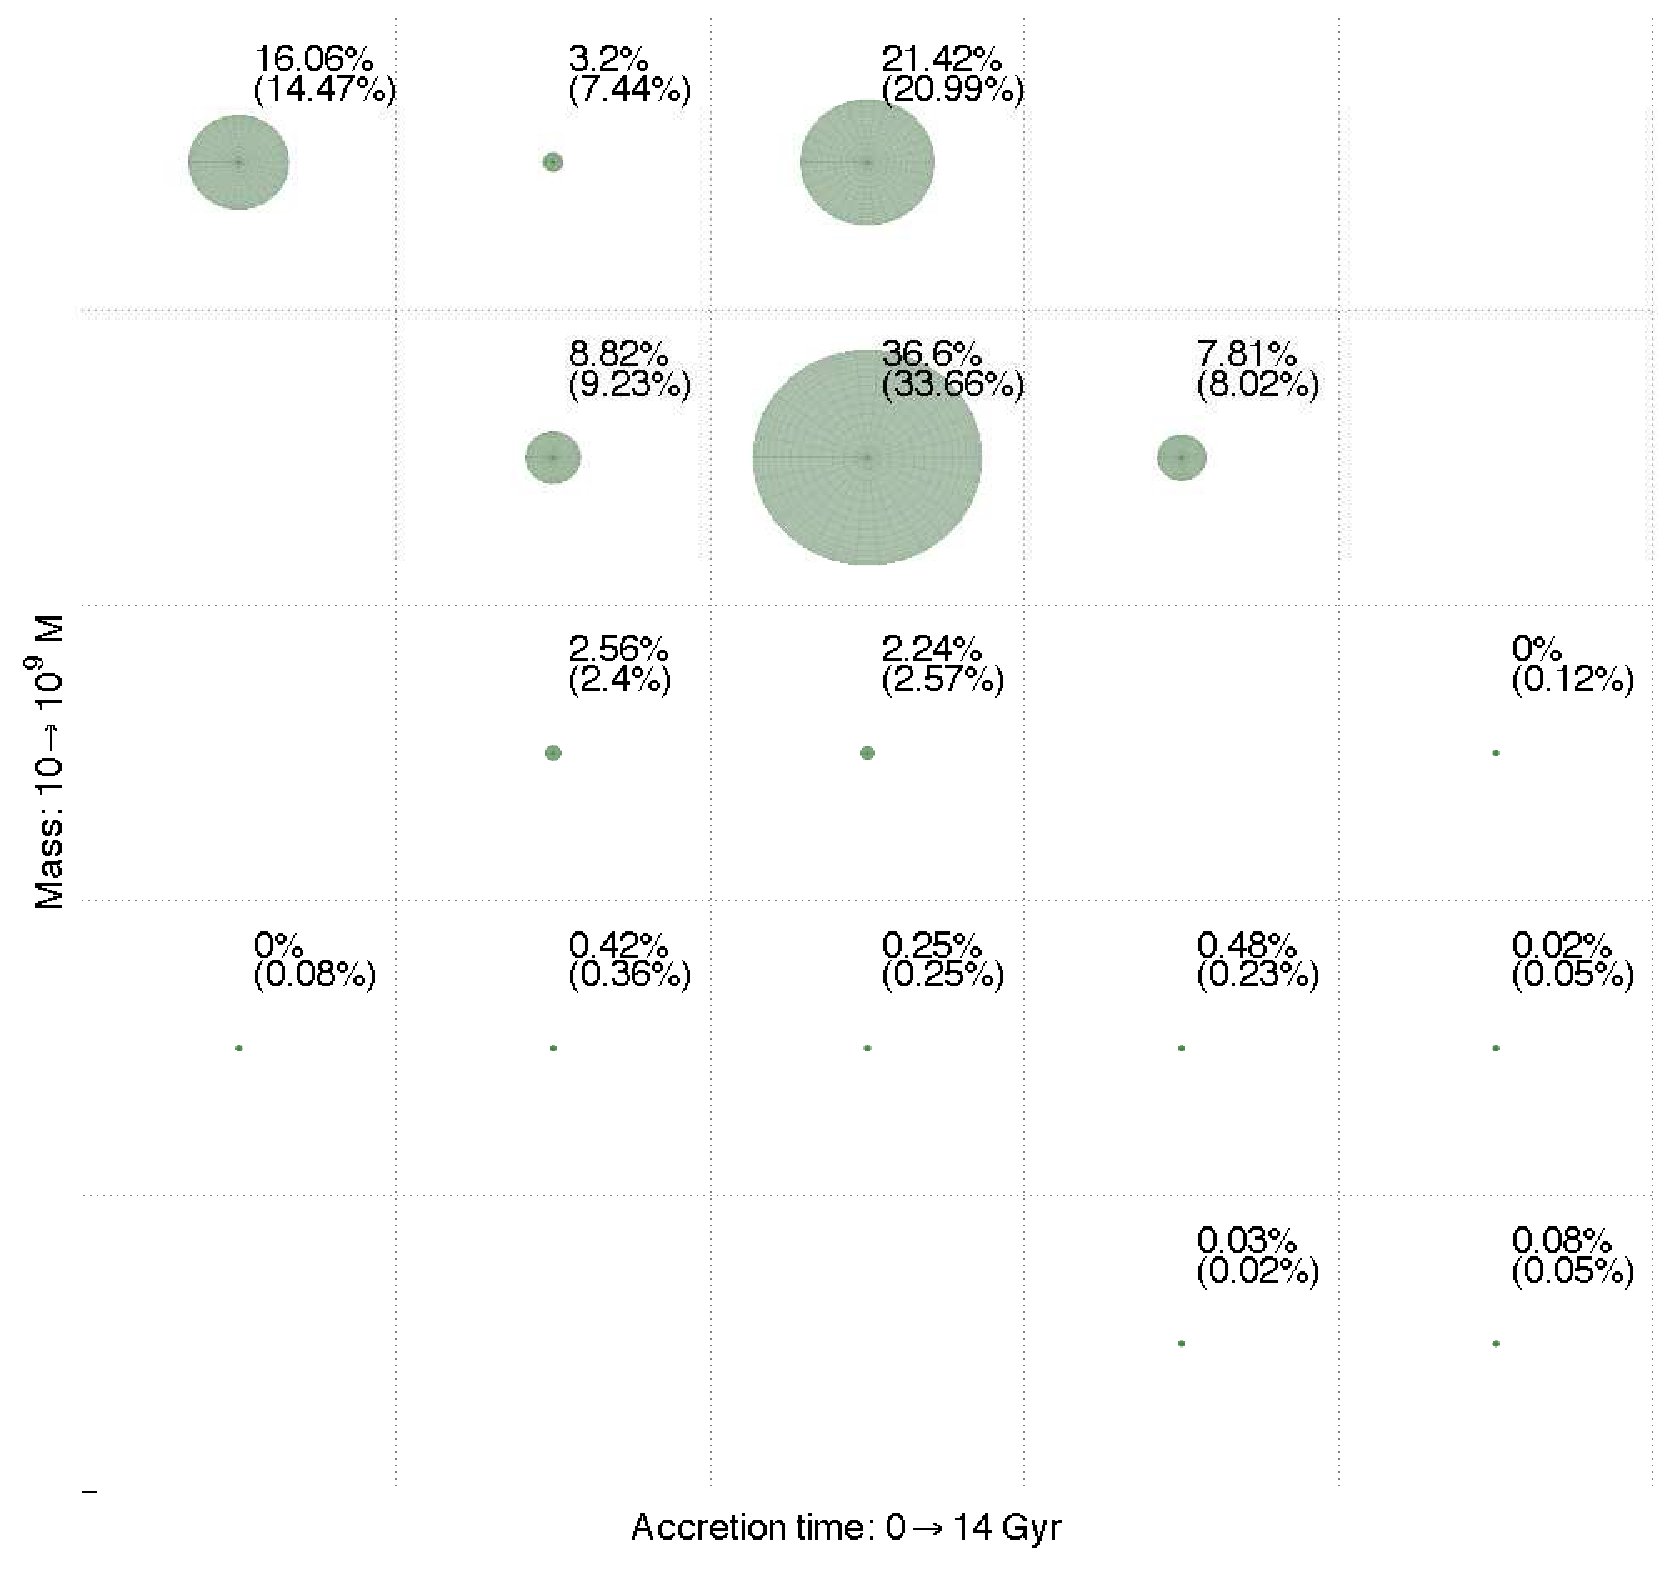
\includegraphics[scale=0.3]{h3fh.pdf}
			\end{center}
	\end{figure}
	
\end{frame}





%%%%%%%%%%%%%%%%%%%%%
\begin{frame}{EM formation history for $m$=4}
	
	\begin{figure}
			\begin{center}
				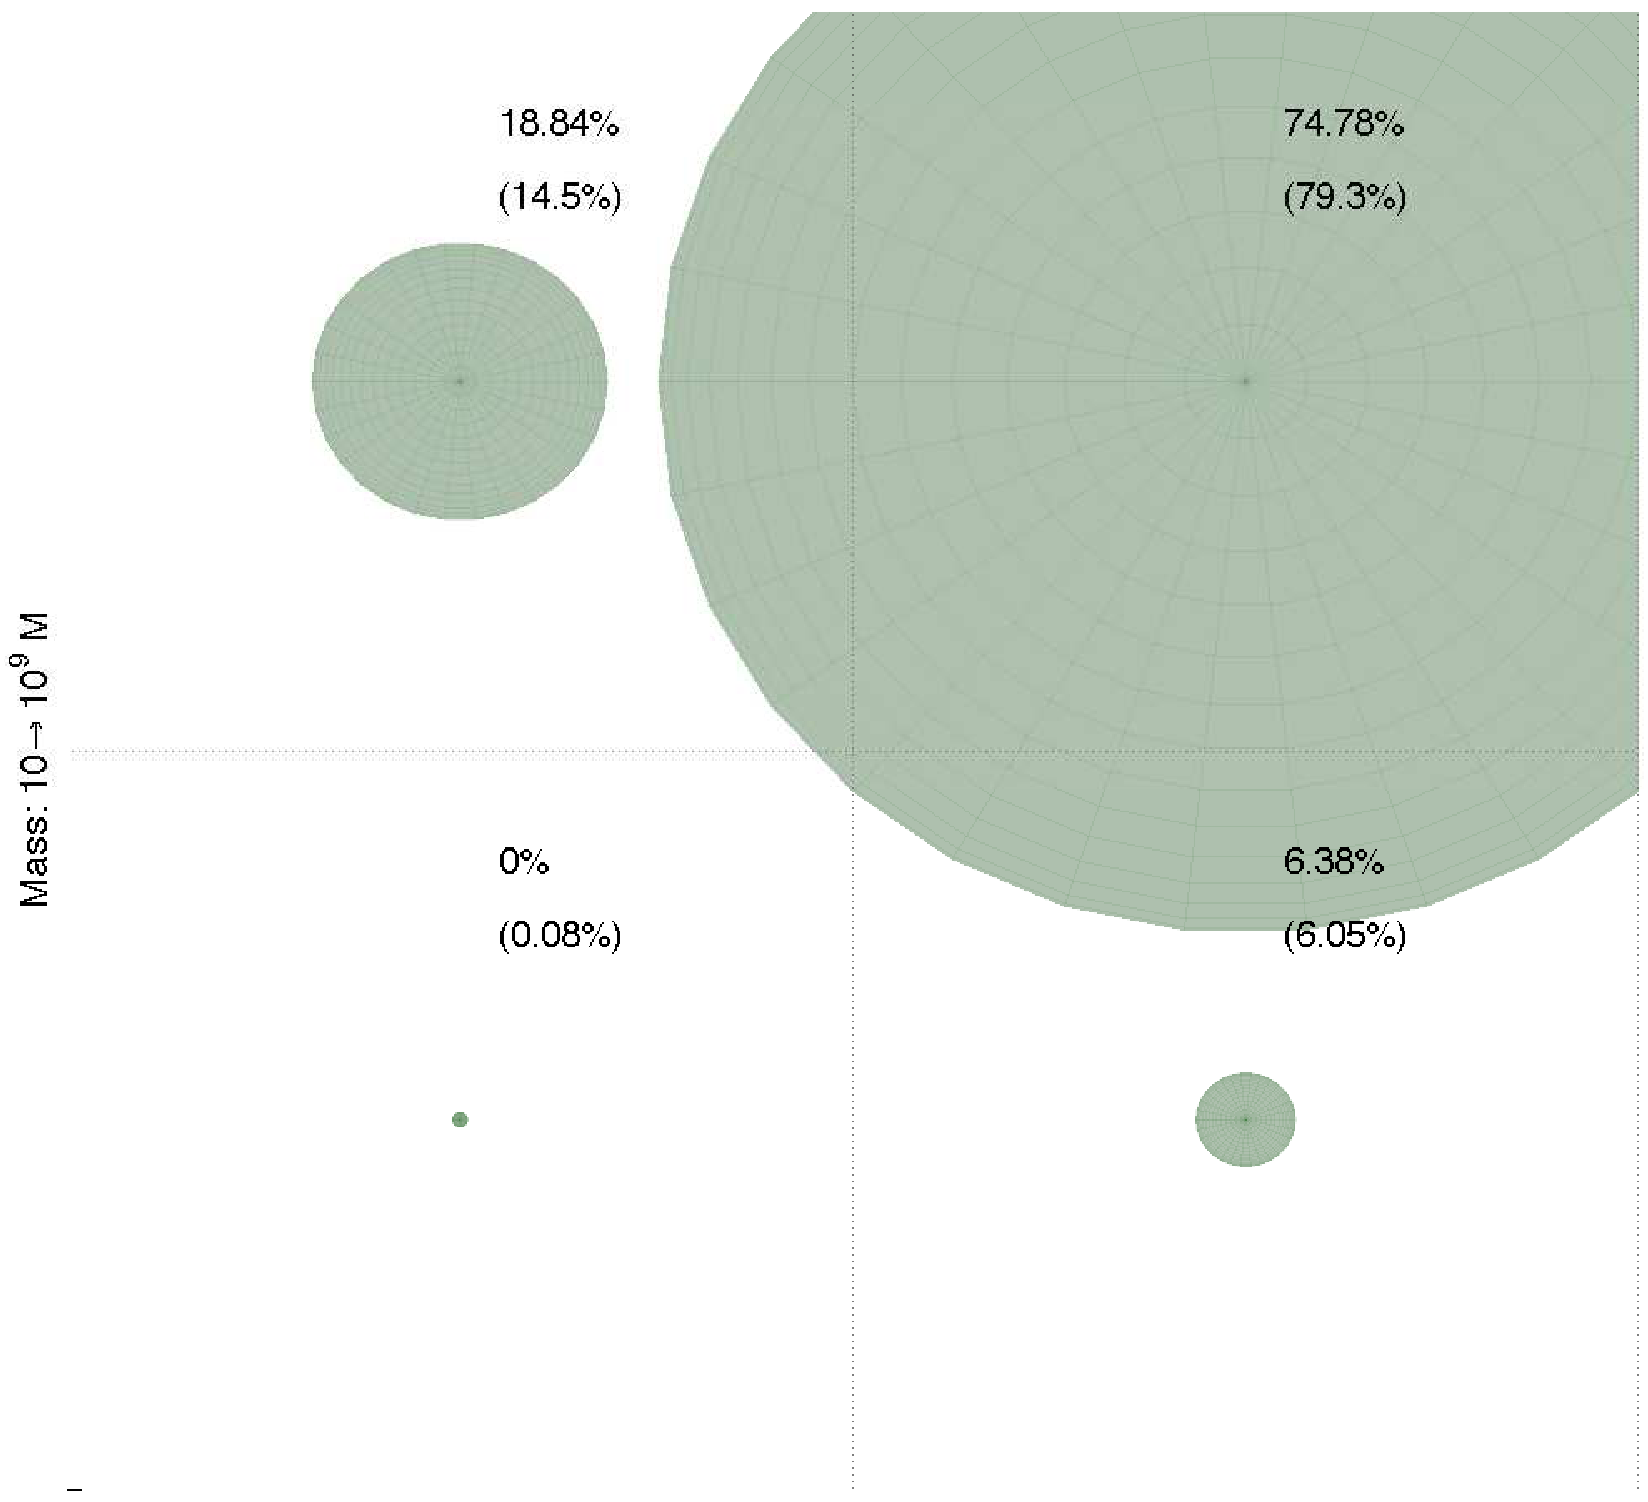
\includegraphics[scale=0.3]{fh2x2.pdf}
			\end{center}
	\end{figure}

	
\end{frame}








%%%%%%%%%%%%%%%%%%%%%
\begin{frame}{Simulation overview}
	
	\begin{figure}
			\begin{center}
				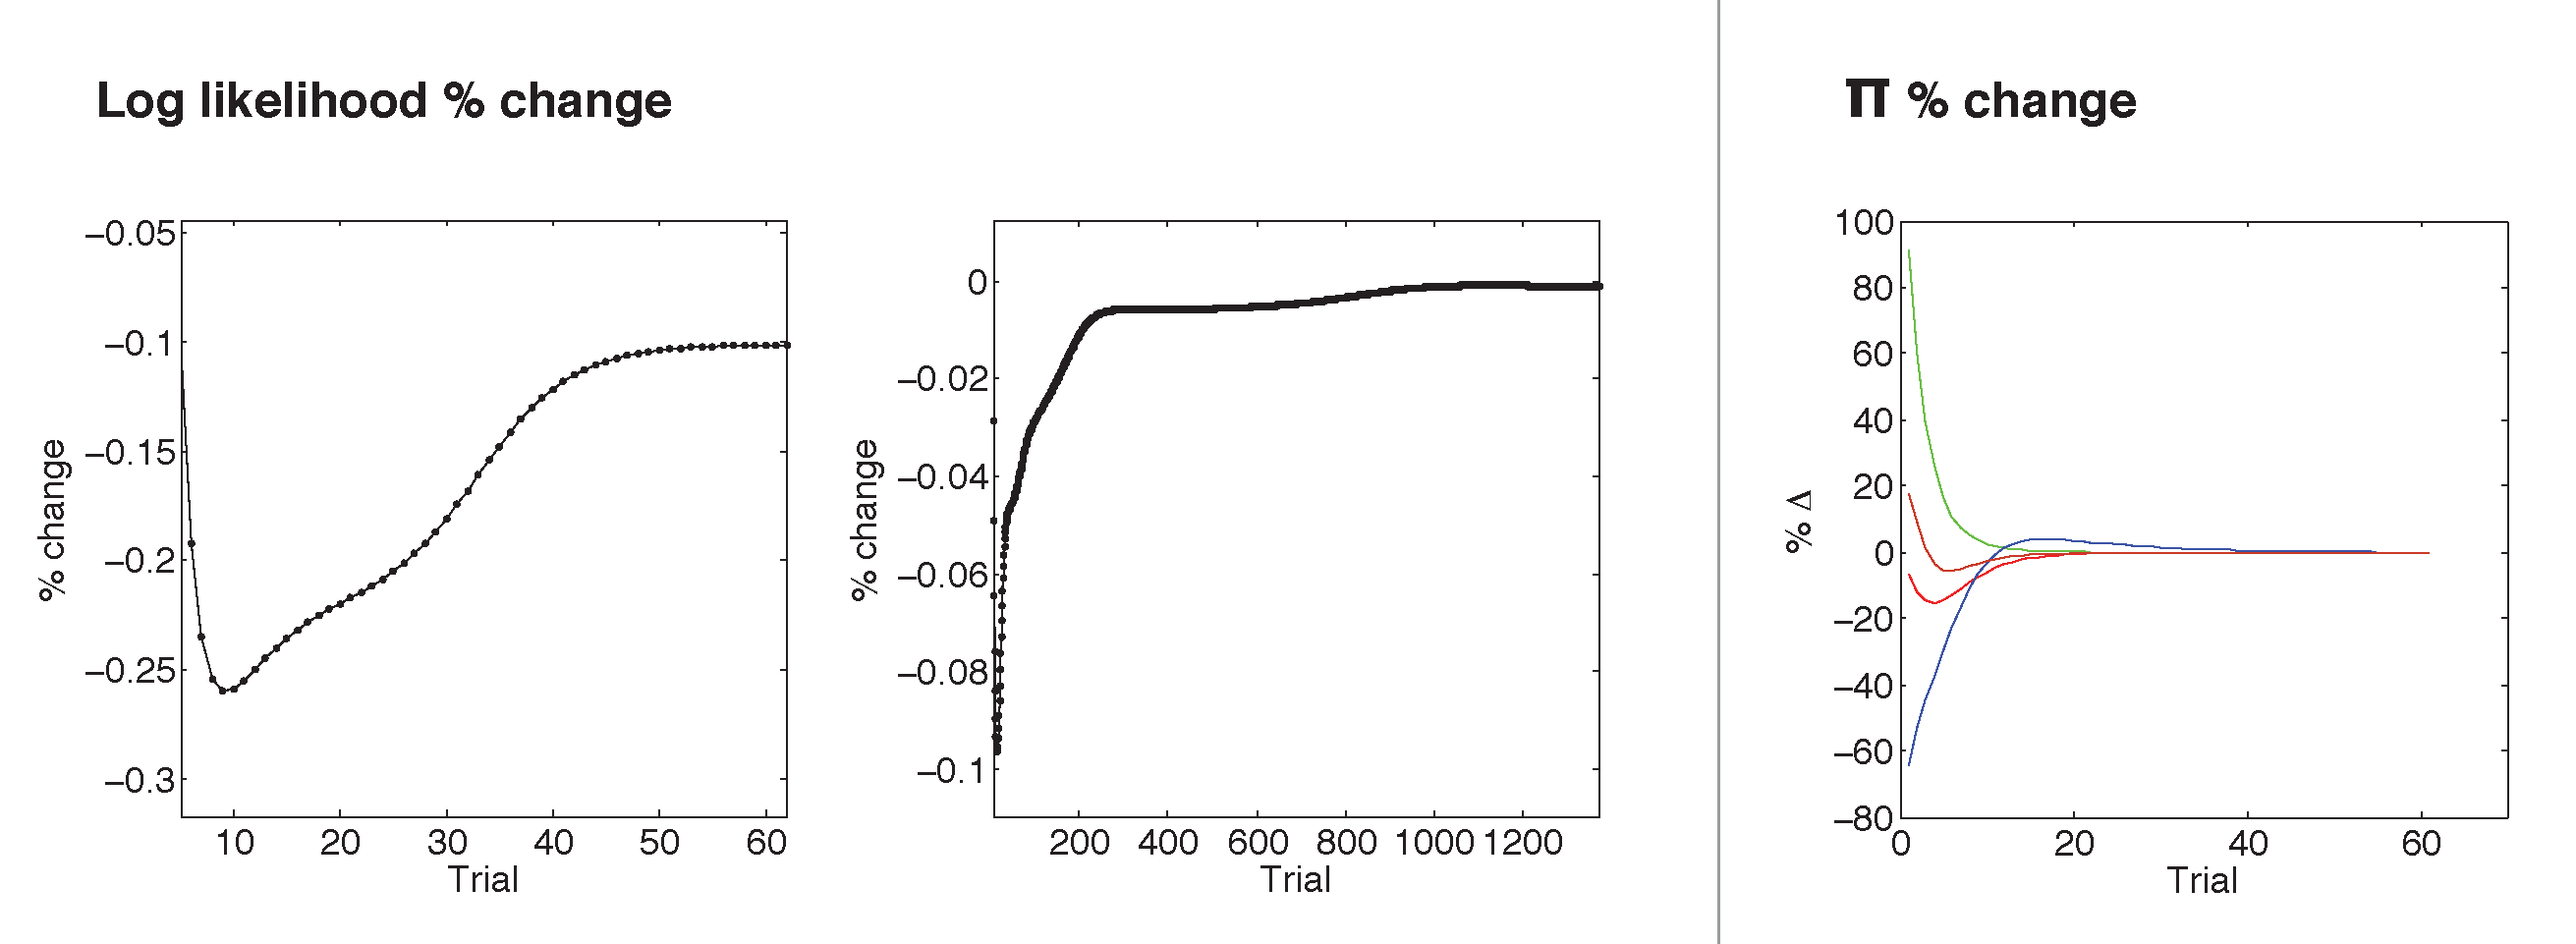
\includegraphics[width=\textwidth]{diag_simple.pdf}
			\end{center}
	\end{figure}
	
	\begin{itemize}
		\item Works with as few as 1,000 observations
		\item Insensitive to initialization of $\vect{\pi}$
		\item Always converges
		\item Large weights identified after 10 iterations
		\item $\llp$ stops changing appreciably after 60 ($m$=4) or 600 ($m$=25) iterations
	\end{itemize}
	
%	1,000 obs, 62 runs, 0.3s m=4
	
%	50,000 obs, 1371 runs, 460s, m=25
	
\end{frame}











%%%%
\begin{frame}{Confidence intervals from observed Fisher Information}
	
	\begin{figure}
			\begin{center}
				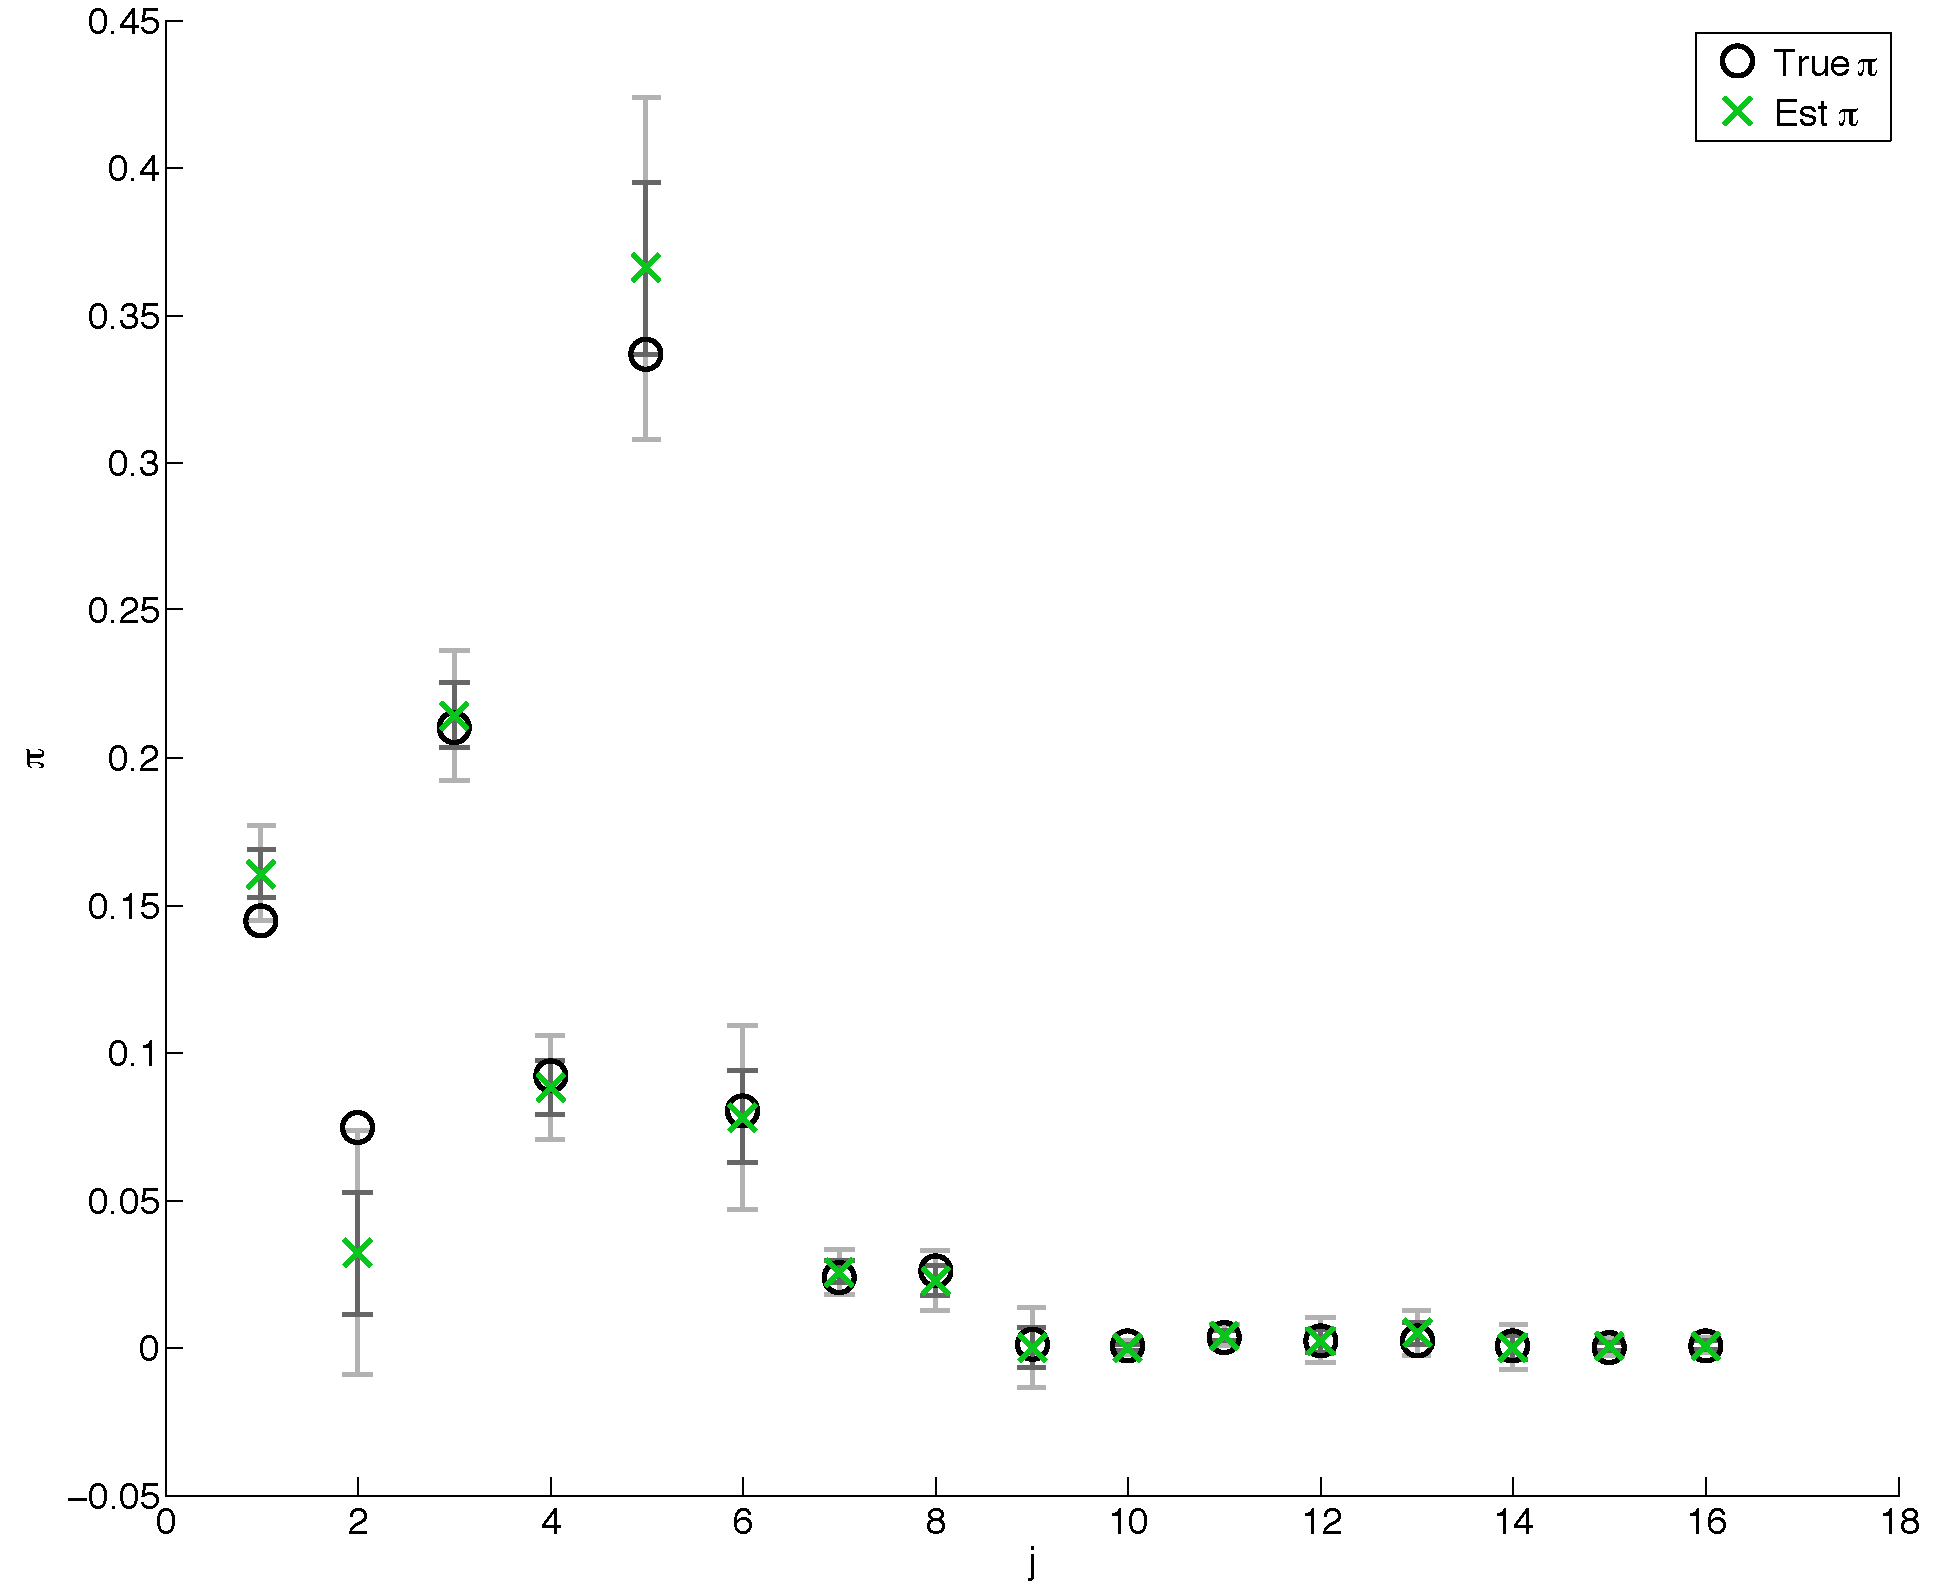
\includegraphics[scale=0.3]{5x5eb.pdf}
			\end{center}
	\end{figure}
	
\end{frame}













%%%%
\begin{frame}{Confidence intervals from observed Fisher Information}
	
	\begin{figure}
			\begin{center}
				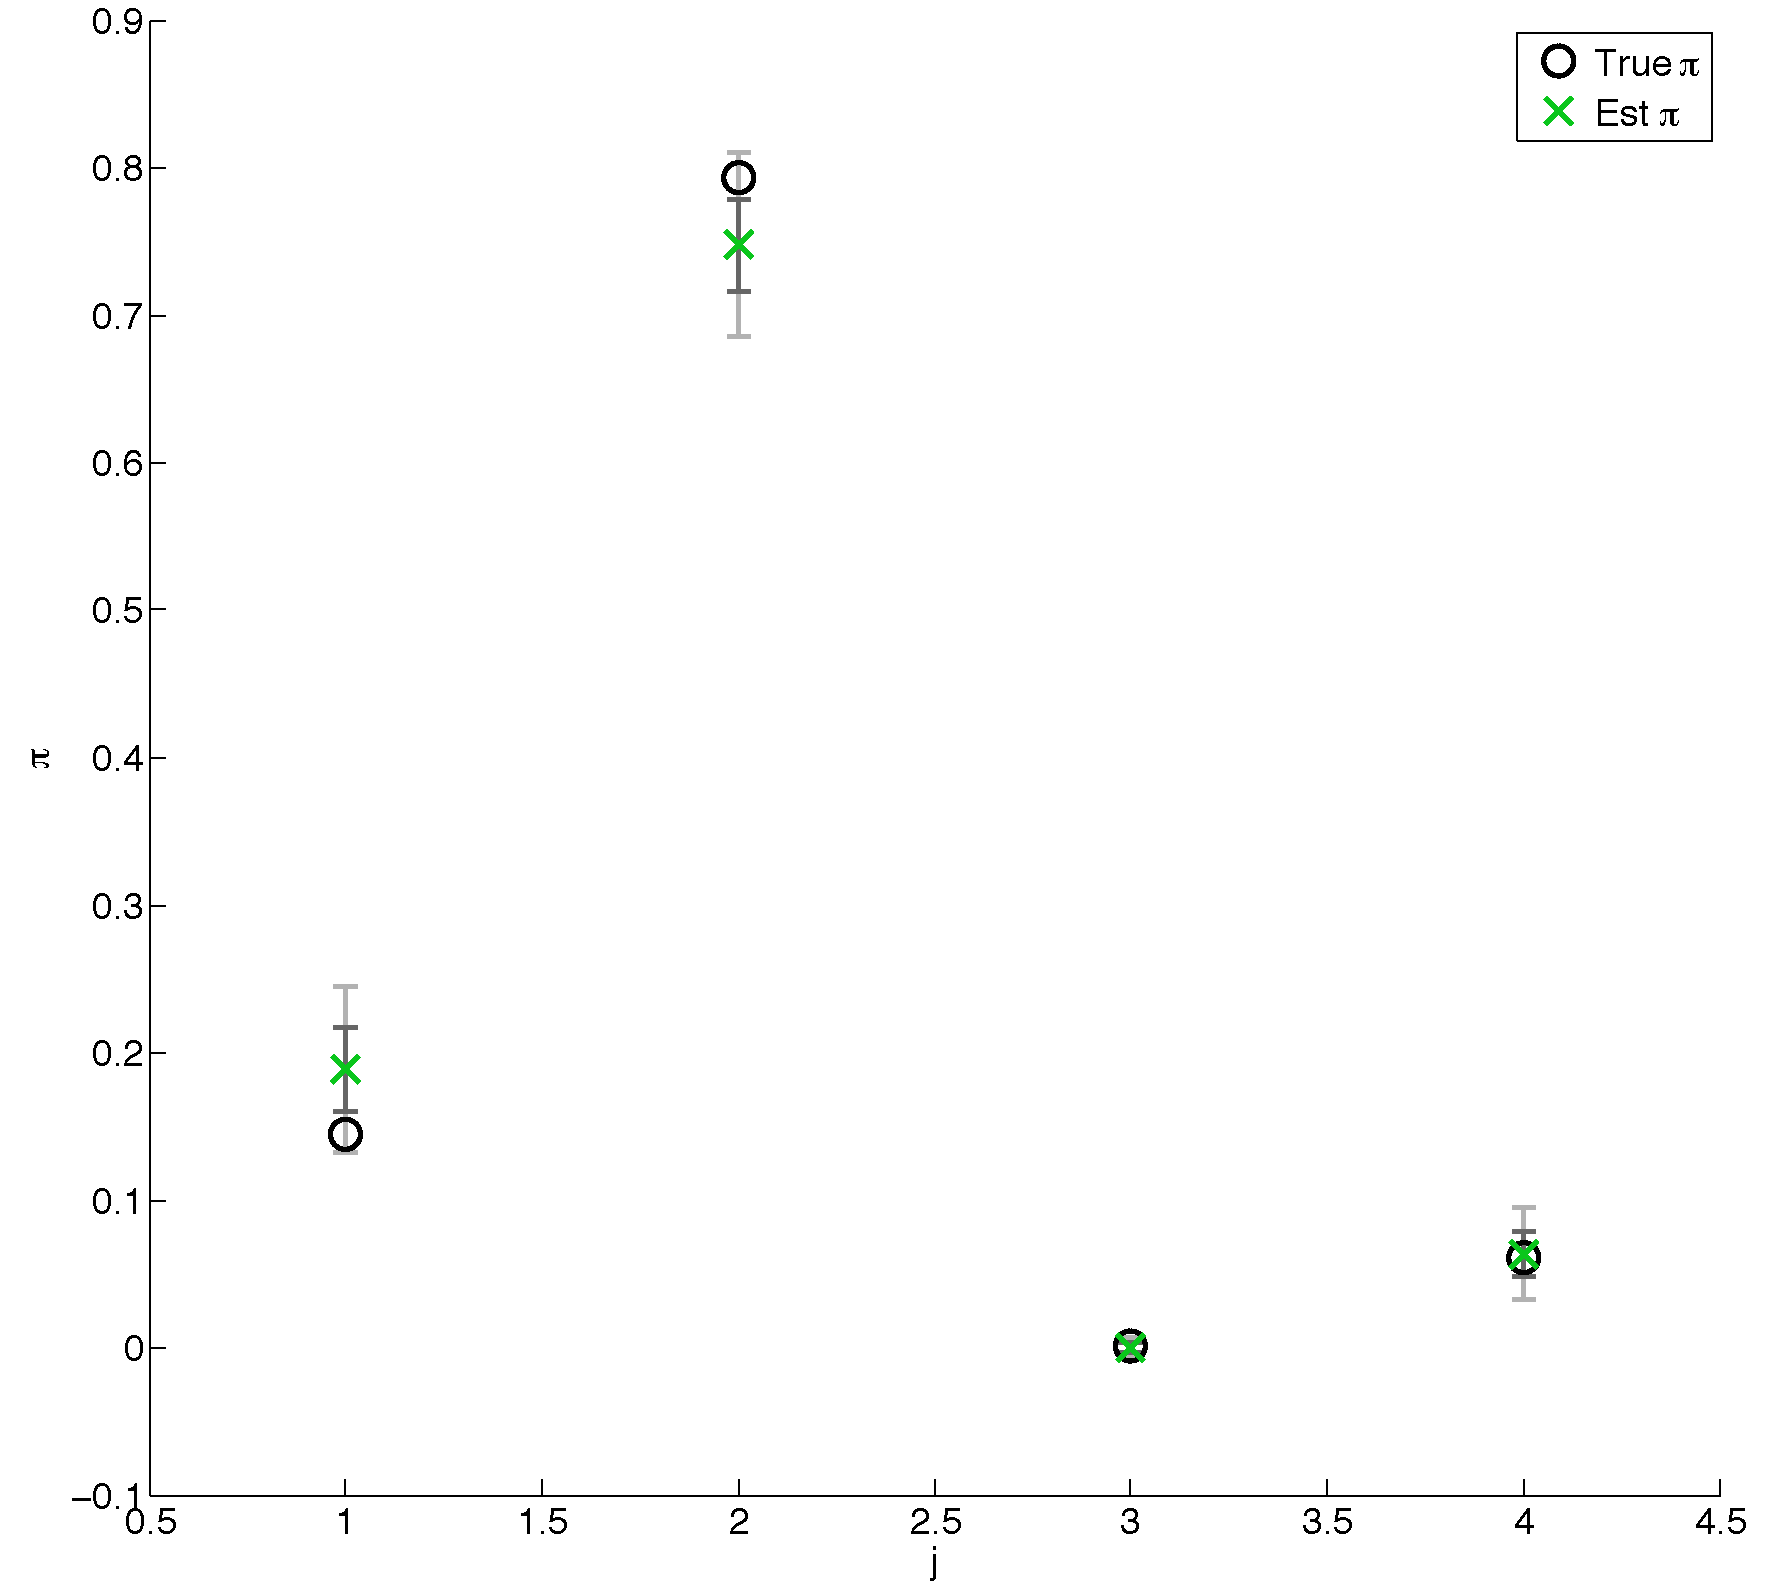
\includegraphics[scale=0.3]{2x2eb.pdf}
			\end{center}
	\end{figure}
	
\end{frame}










%%%%
\begin{frame}{Correlation between $\vp$}
	
	\eqn{	
		I(\vpg|\vx,\vy)=-\frac{\partial^2 \llpp}{\partial \vp^\prime \partial \vp^{\prime T}}
	}		
	
	\begin{figure}
			\begin{center}
				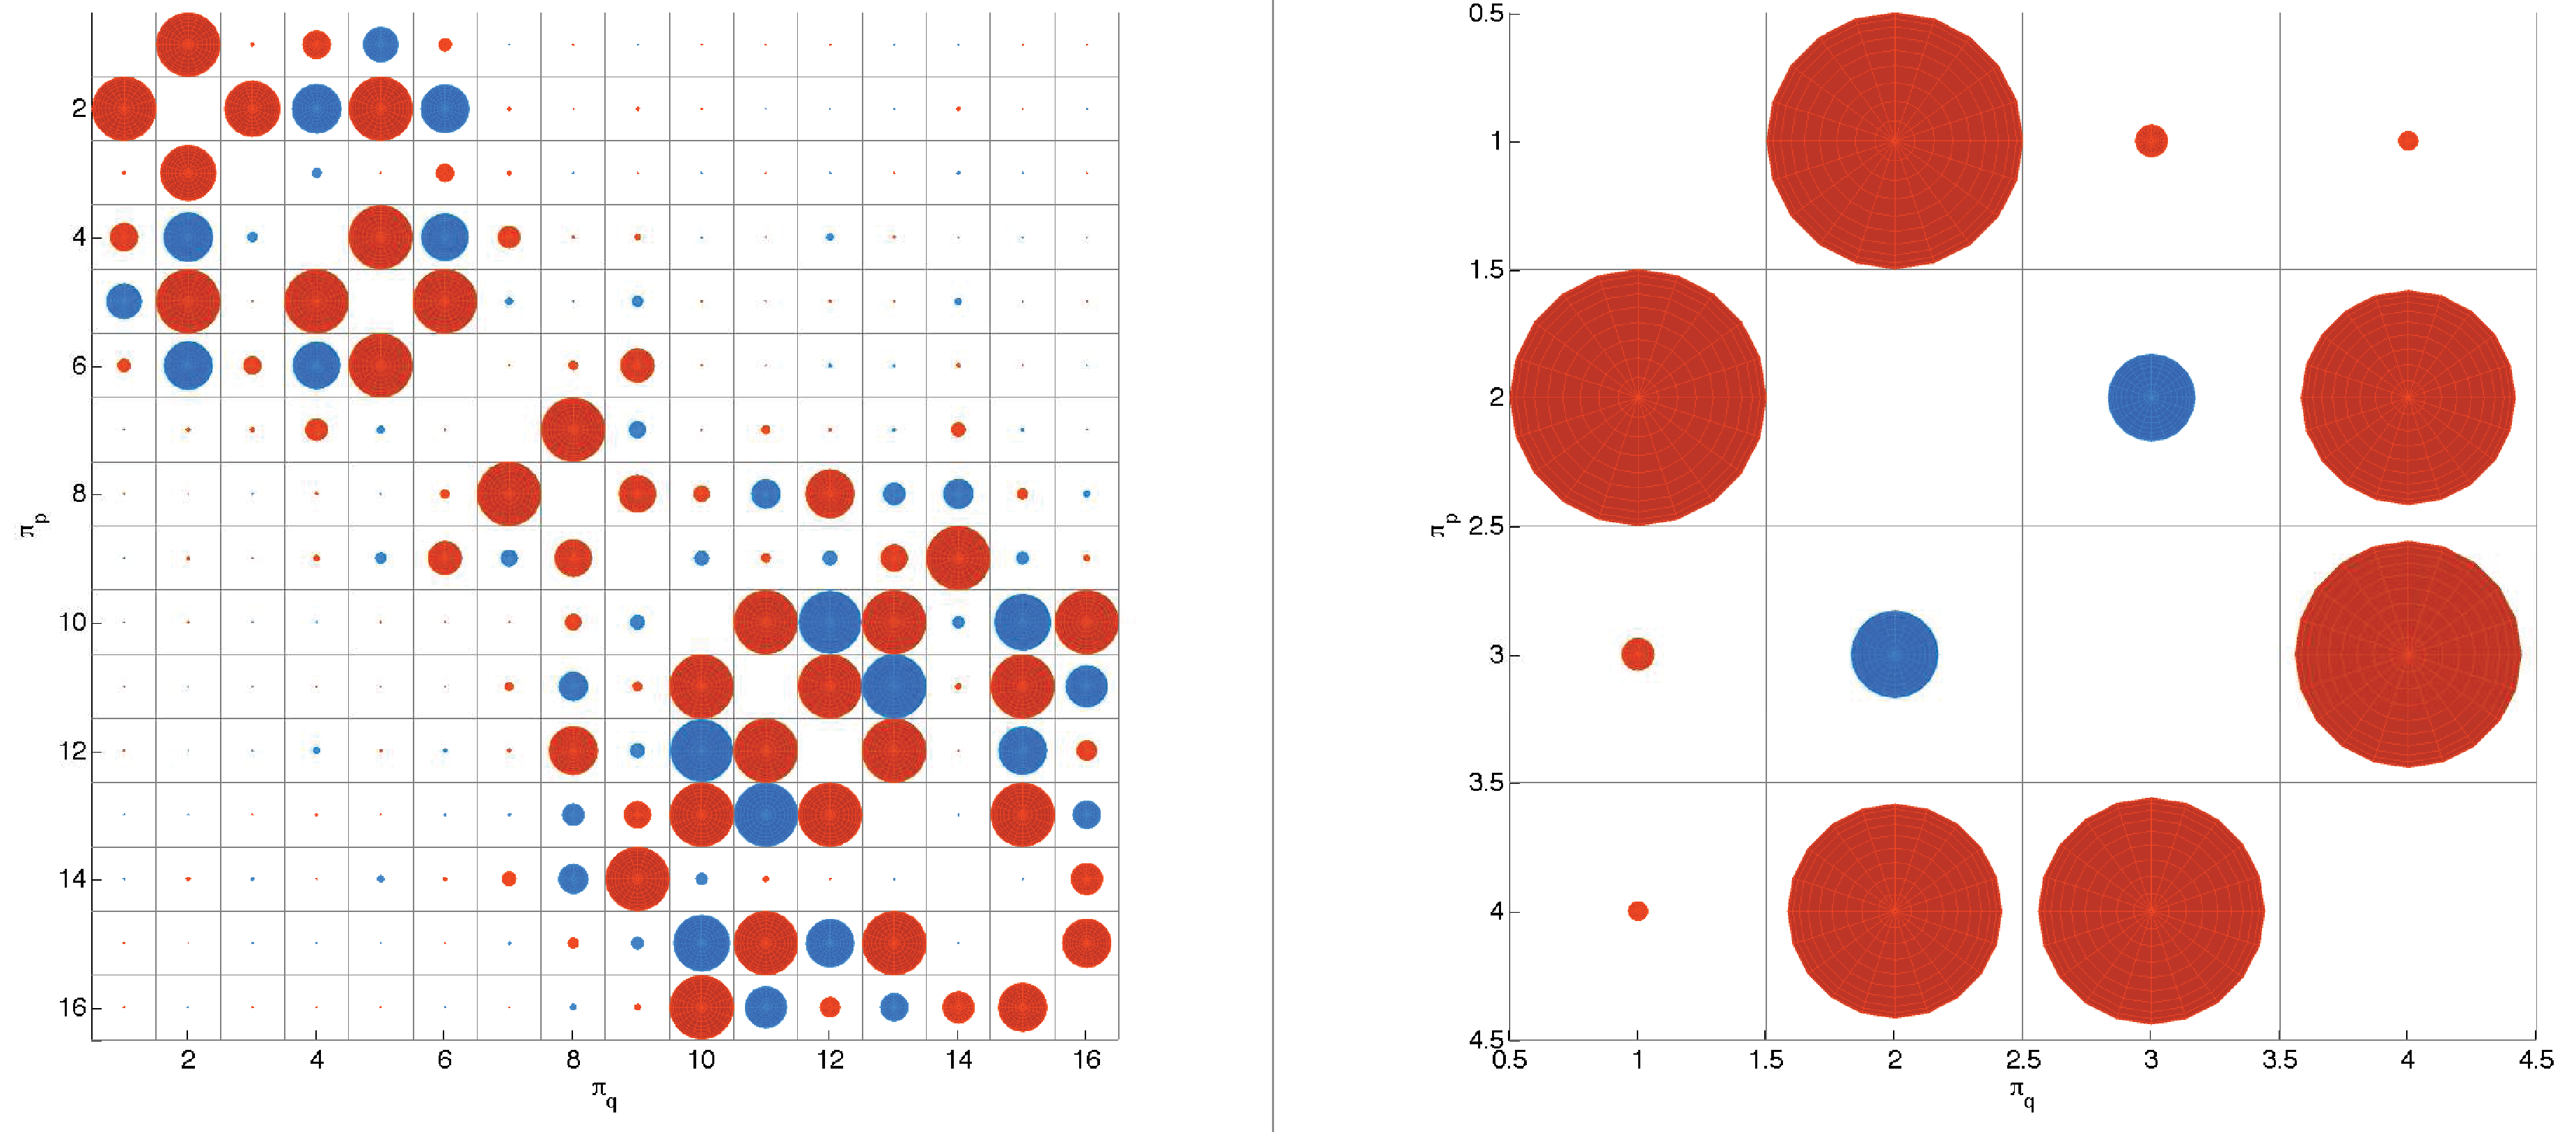
\includegraphics[width=\textwidth]{correl.pdf}
			\end{center}
	\end{figure}	
	
\end{frame}








%%%%
\begin{frame}{Conclusion}
	
	Worked
	\begin{itemize}
		\item 2x2
		\item EM
		\item 5x5 in a few cases
		\item M-of-n bootstrapped errors
	\end{itemize}	
	
	Did not work
	\begin{itemize}
		\item 5x5
		\item Parametric bootstrapped errors
	\end{itemize}	
	
	
	Future improvements
	\begin{itemize}
		\item Non-arbitrary gridding
		\item Smoothing of $f_j$
	\end{itemize}	
	
\end{frame}



































\end{document}


